\hypertarget{test__shorts_8cpp}{}\subsection{test\+\_\+shorts.\+cpp File Reference}
\label{test__shorts_8cpp}\index{test\+\_\+shorts.\+cpp@{test\+\_\+shorts.\+cpp}}


Contains some short examples of performing regex match and regex replace with J\+P\+C\+R\+E2.  


{\ttfamily \#include $<$iostream$>$}\newline
{\ttfamily \#include \char`\"{}jpcre2.\+hpp\char`\"{}}\newline
Include dependency graph for test\+\_\+shorts.\+cpp\+:\nopagebreak
\begin{figure}[H]
\begin{center}
\leavevmode
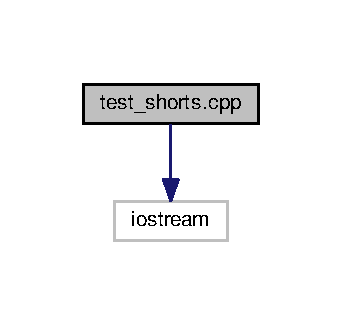
\includegraphics[width=350pt]{test__shorts_8cpp__incl}
\end{center}
\end{figure}


\subsubsection{Detailed Description}
Contains some short examples of performing regex match and regex replace with J\+P\+C\+R\+E2. 


\begin{DoxyCodeInclude}

\textcolor{preprocessor}{#include <iostream>}
\textcolor{preprocessor}{#include "\hyperlink{jpcre2_8hpp}{jpcre2.hpp}"}


\textcolor{keywordtype}{int} main()\{
    \textcolor{keywordtype}{size\_t} count;
    \textcolor{comment}{//Check if string matches the pattern}
    \textcolor{comment}{/*}
\textcolor{comment}{     * The following uses a temporary Regex object.}
\textcolor{comment}{     */}
    \textcolor{keywordflow}{if}(\hyperlink{classjpcre2_1_1Regex}{jpcre2::Regex}(\textcolor{stringliteral}{"(\(\backslash\)\(\backslash\)d)|(\(\backslash\)\(\backslash\)w)"}).match(\textcolor{stringliteral}{"I am the subject"})) 
        std::cout<<\textcolor{stringliteral}{"\(\backslash\)nmatched"};
    \textcolor{keywordflow}{else}
        std::cout<<\textcolor{stringliteral}{"\(\backslash\)nno match"};
    \textcolor{comment}{/*}
\textcolor{comment}{     * Using the modifier S (i.e jpcre2::JIT\_COMPILE) with temporary object may or may not give you}
\textcolor{comment}{     * any performance boost (depends on the complexity of the pattern). The more complex }
\textcolor{comment}{     * the pattern gets, the more sense the S modifier makes.}
\textcolor{comment}{     */}
     
    \textcolor{comment}{//If you want to match all and get the match count, use the action modifier 'g':}
    std::cout<<\textcolor{stringliteral}{"\(\backslash\)n"}<<
        \hyperlink{classjpcre2_1_1Regex}{jpcre2::Regex}(\textcolor{stringliteral}{"(\(\backslash\)\(\backslash\)d)|(\(\backslash\)\(\backslash\)w)"},\textcolor{stringliteral}{"m"}).\hyperlink{classjpcre2_1_1Regex_ab93775a93a0a537d09b9e9ab4a5a3894_ab93775a93a0a537d09b9e9ab4a5a3894}{match}(\textcolor{stringliteral}{"I am the subject"},\textcolor{stringliteral}{"g"});
    
    \textcolor{comment}{/*}
\textcolor{comment}{     * Modifiers passed to the Regex constructor or with compile() function are compile modifiers}
\textcolor{comment}{     * Modifiers passed with the match() or replace() functions are action modifiers}
\textcolor{comment}{     */}
    
    \textcolor{comment}{// Substrings/Captured groups:}
    
    \textcolor{comment}{/*}
\textcolor{comment}{     * *** Getting captured groups/substring ***}
\textcolor{comment}{     * }
\textcolor{comment}{     * captured groups or substrings are stored in maps for each match,}
\textcolor{comment}{     * and each match is stored in a vector. }
\textcolor{comment}{     * Thus captured groups are in a vector of maps.}
\textcolor{comment}{     * }
\textcolor{comment}{     * PCRE2 provides two types of substrings:}
\textcolor{comment}{     *  1. numbered (index) substring}
\textcolor{comment}{     *  2. named substring}
\textcolor{comment}{     * }
\textcolor{comment}{     * For the above two, we have two vectors respectively:}
\textcolor{comment}{     *  1. jpcre2::VecNum (Corresponding map: jpcre2::MapNum)}
\textcolor{comment}{     *  2. jpcre2::VecNas (Corresponding map: jpcre2::MapNas)}
\textcolor{comment}{     * }
\textcolor{comment}{     * Another additional vector is available to get the substring position/number}
\textcolor{comment}{     * for a particular captured group by name. It's a vector of name to number maps}
\textcolor{comment}{     *  * jpcre2::VecNtN (Corresponding map: jpcre2:MapNtN)}
\textcolor{comment}{     */}
    
    \textcolor{comment}{// ***** Get numbered substring ***** ///}
    \hyperlink{namespacejpcre2_ac1cf752c8fbb0be78020be3b80e77ce3}{jpcre2::VecNum} vec\_num;
    count = 
    \hyperlink{classjpcre2_1_1Regex}{jpcre2::Regex}(\textcolor{stringliteral}{"(\(\backslash\)\(\backslash\)w+)\(\backslash\)\(\backslash\)s*(\(\backslash\)\(\backslash\)d+)"},\textcolor{stringliteral}{"m"})
            .\hyperlink{classjpcre2_1_1Regex_a519b0915bf1163c6ce6a4d674b30cfcd_a519b0915bf1163c6ce6a4d674b30cfcd}{initMatch}()
            .\hyperlink{classjpcre2_1_1RegexMatch_a635c652195deaa8ebb9e107c4f972aab_a635c652195deaa8ebb9e107c4f972aab}{setSubject}(\textcolor{stringliteral}{"I am 23, I am digits 10"})
            .\hyperlink{classjpcre2_1_1RegexMatch_a9df7e92f96b61553f62720cb8f5f23e5_a9df7e92f96b61553f62720cb8f5f23e5}{setModifier}(\textcolor{stringliteral}{"g"})
            .\hyperlink{classjpcre2_1_1RegexMatch_a2c7efe1ec2e13827f670db4ecedcd0a0_a2c7efe1ec2e13827f670db4ecedcd0a0}{setNumberedSubstringVector}(&vec\_num)
            .\hyperlink{classjpcre2_1_1RegexMatch_a5868aef3a146594ea1ebef34d122bb33_a5868aef3a146594ea1ebef34d122bb33}{match}();
    \textcolor{comment}{/*}
\textcolor{comment}{    * count (the return value) is guaranteed to give you the correct number of matches,}
\textcolor{comment}{    * while vec\_num.size() may give you wrong result if any match result}
\textcolor{comment}{    * was failed to be inserted in the vector. This should not happen}
\textcolor{comment}{    * i.e count and vec\_num.size() should always be equal.}
\textcolor{comment}{    */}
    std::cout<<\textcolor{stringliteral}{"\(\backslash\)nNumber of matches: "}<<count\textcolor{comment}{/* or vec\_num.size()*/};

    \textcolor{comment}{//Now vec\_num is populated with numbered substrings for each match}
    \textcolor{comment}{//The size of vec\_num is the total match count}
    \textcolor{comment}{//vec\_num[0] is the first match}
    \textcolor{comment}{//The type of vec\_num[0] is jpcre2::MapNum}
    std::cout<<\textcolor{stringliteral}{"\(\backslash\)nTotal match of first match: "}<<vec\_num[0][0];      
    std::cout<<\textcolor{stringliteral}{"\(\backslash\)nCaptrued group 1 of first match: "}<<vec\_num[0][1]; 
    std::cout<<\textcolor{stringliteral}{"\(\backslash\)nCaptrued group 2 of first match: "}<<vec\_num[0][2]; 
    
     \textcolor{comment}{//captured group 3 doesn't exist, it will give you empty string}
    std::cout<<\textcolor{stringliteral}{"\(\backslash\)nCaptrued group 3 of first match: "}<<vec\_num[0][3];
    
    \textcolor{comment}{//Using the [] operator with jpcre2::MapNum will create new element if it doesn't exist}
    \textcolor{comment}{// i.e vec\_num[0][3] were created in the above example.}
    \textcolor{comment}{//This should be ok, if existence of a particular substring is not important}

    \textcolor{comment}{//If the existence of a substring is important, use the std::map::find() or std::map::at() (>=C++11)
       function to access map elements}
    \textcolor{comment}{/* //>=C++11}
\textcolor{comment}{    try\{}
\textcolor{comment}{        //This will throw exception, because substring 4 doesn't exist}
\textcolor{comment}{        std::cout<<"\(\backslash\)nCaptrued group 4 of first match: "<<vec\_num[0].at(4);}
\textcolor{comment}{    \} catch (std::logic\_error& e)\{}
\textcolor{comment}{        std::cerr<<"\(\backslash\)nCaptrued group 4 doesn't exist";}
\textcolor{comment}{    \}*/}
    
    \textcolor{comment}{//There were two matches found (vec\_num.size() == 2) in the above example}
    std::cout<<\textcolor{stringliteral}{"\(\backslash\)nTotal match of second match: "}<<vec\_num[1][0];      \textcolor{comment}{//Total match (group 0) from second
       match}
    std::cout<<\textcolor{stringliteral}{"\(\backslash\)nCaptrued group 1 of second match: "}<<vec\_num[1][1]; \textcolor{comment}{//captured group 1 from second match }
    std::cout<<\textcolor{stringliteral}{"\(\backslash\)nCaptrued group 2 of second match: "}<<vec\_num[1][2]; \textcolor{comment}{//captured group 2 from second match}
    
    
    \textcolor{comment}{// ***** Get named substring ***** //}
    
    \hyperlink{namespacejpcre2_a2b121ae776ea5b2913839f418a7d856b}{jpcre2::VecNas} vec\_nas;
    \hyperlink{namespacejpcre2_a88a7aaf84cad627d34c8152e726168eb}{jpcre2::VecNtN} vec\_ntn; \textcolor{comment}{// We will get name to number map vector too}
    count = 
    \hyperlink{classjpcre2_1_1Regex}{jpcre2::Regex}(\textcolor{stringliteral}{"(?<word>\(\backslash\)\(\backslash\)w+)\(\backslash\)\(\backslash\)s*(?<digit>\(\backslash\)\(\backslash\)d+)"},\textcolor{stringliteral}{"m"})
            .\hyperlink{classjpcre2_1_1Regex_a519b0915bf1163c6ce6a4d674b30cfcd_a519b0915bf1163c6ce6a4d674b30cfcd}{initMatch}()
            .\hyperlink{classjpcre2_1_1RegexMatch_a635c652195deaa8ebb9e107c4f972aab_a635c652195deaa8ebb9e107c4f972aab}{setSubject}(\textcolor{stringliteral}{"I am 23, I am digits 10"})
            .\hyperlink{classjpcre2_1_1RegexMatch_a9df7e92f96b61553f62720cb8f5f23e5_a9df7e92f96b61553f62720cb8f5f23e5}{setModifier}(\textcolor{stringliteral}{"g"})
            \textcolor{comment}{//.setNumberedSubstringVector(vec\_num) // We don't need it in this example}
            .\hyperlink{classjpcre2_1_1RegexMatch_ae495431f57cae54363331237ab21b56c_ae495431f57cae54363331237ab21b56c}{setNamedSubstringVector}(&vec\_nas)
            .\hyperlink{classjpcre2_1_1RegexMatch_a04926e61d8b5f1d8bdf344efecd567d8_a04926e61d8b5f1d8bdf344efecd567d8}{setNameToNumberMapVector}(&vec\_ntn) \textcolor{comment}{// Additional (name to number maps)}
            .\hyperlink{classjpcre2_1_1RegexMatch_a5868aef3a146594ea1ebef34d122bb33_a5868aef3a146594ea1ebef34d122bb33}{match}();
    std::cout<<\textcolor{stringliteral}{"\(\backslash\)nNumber of matches: "}<<vec\_nas.size()\textcolor{comment}{/* or count */};
    \textcolor{comment}{//Now vec\_nas is populated with named substrings for each match}
    \textcolor{comment}{//The size of vec\_nas is the total match count}
    \textcolor{comment}{//vec\_nas[0] is the first match}
    \textcolor{comment}{//The type of vec\_nas[0] is jpcre2::MapNas}
    std::cout<<\textcolor{stringliteral}{"\(\backslash\)nCaptured group (word) of first match: "}<<vec\_nas[0][\textcolor{stringliteral}{"word"}];
    std::cout<<\textcolor{stringliteral}{"\(\backslash\)nCaptured group (digit) of first match: "}<<vec\_nas[0][\textcolor{stringliteral}{"digit"}];
    
    \textcolor{comment}{//If the existence of a substring is important, use the std::map::find() or std::map::at() (>=C++11)
       function to access map elements}
    \textcolor{comment}{/* //>=C++11}
\textcolor{comment}{    try\{}
\textcolor{comment}{        std::cout<<"\(\backslash\)nCaptured group (name) of first match: "<<vec\_nas[0].at("name");}
\textcolor{comment}{    \} catch(std::logic\_error& e)\{}
\textcolor{comment}{        std::cerr<<"\(\backslash\)nCaptured group (name) doesn't exist";}
\textcolor{comment}{    \}*/}
    
    \textcolor{comment}{//There were two matches found (vec\_nas.size() == 2) in the above example}
    std::cout<<\textcolor{stringliteral}{"\(\backslash\)nCaptured group (word) of second match: "}<<vec\_nas[1][\textcolor{stringliteral}{"word"}];
    std::cout<<\textcolor{stringliteral}{"\(\backslash\)nCaptured group (digit) of second match: "}<<vec\_nas[1][\textcolor{stringliteral}{"digit"}];

    \textcolor{comment}{//Get the position (number) of a captured group name (that was found in match)}
    std::cout<<\textcolor{stringliteral}{"\(\backslash\)nPosition of captured group (word) in first match: "}<<vec\_ntn[0][\textcolor{stringliteral}{"word"}];
    std::cout<<\textcolor{stringliteral}{"\(\backslash\)nPosition of captured group (digit) in first match: "}<<vec\_ntn[0][\textcolor{stringliteral}{"digit"}];
    
    \textcolor{comment}{/*}
\textcolor{comment}{     * Replacement Examples}
\textcolor{comment}{     * Replace pattern in a string with a replacement string}
\textcolor{comment}{     * }
\textcolor{comment}{     * The initReplace() function can take a subject and replacement string as argument.}
\textcolor{comment}{     * You can also pass the subject with setSubject() function in method chain,}
\textcolor{comment}{     * replacement string with setReplaceWith() function in method chain, etc ...}
\textcolor{comment}{     * }
\textcolor{comment}{     * A call to replace() will return the resultant string}
\textcolor{comment}{     */}
    
    std::cout<<\textcolor{stringliteral}{"\(\backslash\)n"}<<
    \textcolor{comment}{//replace first occurrence of a digit with @}
    \hyperlink{classjpcre2_1_1Regex}{jpcre2::Regex}(\textcolor{stringliteral}{"\(\backslash\)\(\backslash\)d"}).\hyperlink{classjpcre2_1_1Regex_ac592ce7a5e4210ed5f90a0105b1f2981_ac592ce7a5e4210ed5f90a0105b1f2981}{replace}(\textcolor{stringliteral}{"I am the subject string 44"}, \textcolor{stringliteral}{"@"});
    
    std::cout<<\textcolor{stringliteral}{"\(\backslash\)n"}<<
    \textcolor{comment}{//replace all occurrences of a digit with @}
    \hyperlink{classjpcre2_1_1Regex}{jpcre2::Regex}(\textcolor{stringliteral}{"\(\backslash\)\(\backslash\)d"}).\hyperlink{classjpcre2_1_1Regex_ac592ce7a5e4210ed5f90a0105b1f2981_ac592ce7a5e4210ed5f90a0105b1f2981}{replace}(\textcolor{stringliteral}{"I am the subject string 44"}, \textcolor{stringliteral}{"@"}, \textcolor{stringliteral}{"g"});
    
    \textcolor{comment}{//swap two parts of a string}
    std::cout<<\textcolor{stringliteral}{"\(\backslash\)n"}<<
    \hyperlink{classjpcre2_1_1Regex}{jpcre2::Regex}(\textcolor{stringliteral}{"^([^\(\backslash\)t]+)\(\backslash\)t([^\(\backslash\)t]+)$"})
            .\hyperlink{classjpcre2_1_1Regex_ac592ce7a5e4210ed5f90a0105b1f2981_ac592ce7a5e4210ed5f90a0105b1f2981}{replace}(\textcolor{stringliteral}{"I am the subject\(\backslash\)tTo be swapped according to tab"}, \textcolor{stringliteral}{"$2 $1"});
            

    \textcolor{keywordflow}{return} 0;
\}
\end{DoxyCodeInclude}
 \begin{DoxyAuthor}{Author}
\href{https://github.com/neurobin}{\tt Md Jahidul Hamid} 
\end{DoxyAuthor}
